%!TEX root =  ../master.tex
\section{One Dimension}\label{sec:1D}
For completeness we also provide a discussion for L\"uscher's formula in one dimension with a contact interaction.  Plugging in $D=1$ into eqs.~\eqref{general luscher}, \eqref{I0 FV}, and~\eqref{spherical FD}, and noting that $\mathcal{L}_{D=1}^\bigcirc=0$, one finds 
\begin{align} 
C(\Lambda)&=-\frac{1}{\mu a_{10}}\\
\frac{a_{10}}{L} &=\frac{1}{2 \pi^{2}} \sum_{n=-\infty}^{\infty} \frac{1}{n^{2}-\left(\frac{p L}{2 \pi}\right)^{2}} \\ 
& \equiv \frac{1}{2 \pi^{2}} S_{1}\left(\left(\frac{p L}{2 \pi^{2}}\right)^{2}\right)\ .
\end{align}
In one dimension the sum in the zeta function is well behaved and has a compact form,
\begin{equation}
S^\bigcirc_{1}(x) \equiv \sum_{n=-\infty}^{\infty} \frac{1}{n^{2}-x}=-\pi \frac{\cot (\pi \sqrt{x})}{\sqrt{x}}\ ,
\end{equation}
which gives a closed form expression for L\"uscher's formula,
\begin{equation}\label{eq:1d luscher}
\frac{a_{10}}{L} =-\frac{1}{pL}\cot\left(\frac{pL}{2}\right)\ . 
\end{equation}
Our result is consistent with those found in \cite{}.

Since no cutoff is required in one dimension, the dispersion form of L\"uscher's formula is straightforward to obtain.  If one identifies the lattice spacing as a cutoff, i.e. $\epsilon = N/L$, then the sum in the zeta function is restricted to the Brillouin zone and one has
\begin{align}
 \frac{a_{10}}{L} &=\frac{1}{2 \pi^{2}} \sum_{n=-\frac{N}{2}}^{\frac{N}{2}-1} \frac{1}{n^{2}-\left(\frac{p L}{2 \pi}\right)^{2}} \\
 & \equiv \frac{1}{2 \pi^{2}} S^{\dispersion}_{1}\left(\left(\frac{p L}{2 \pi^{2}}\right)^{2}\right)\ .\label{eq:1d dispersion}
 \end{align}
 Here we assumed $n_s=\infty$.  
Eigenvalues $p^2/m$ of Schr\"odinger's equation on a discretized torus will satisfy the relation in eq.~\eqref{1d dispersion}.  As stressed in the previous section, only continuum extracted eigenvalues should be used in eq.~\eqref{1d luscher}, otherwise induced momentum-dependent terms will occur.  For example, in \autoref{fig:luescher1d} we show  the effects of the induced momentum-dependent terms when non-continuum eigenvalues are inserted into $S^\bigcirc_1(x)$ (colored points) for lattice sizes of $N=10$, 12, and 14.  The non-flat behavior expected of a momentum-dependent interaction is apparent.  Included in the figure are also the points determined from the $S^{\dispersion}_1(x)$ (black points), and these all lie on a flat line, as expected.  
\begin{figure}
\center
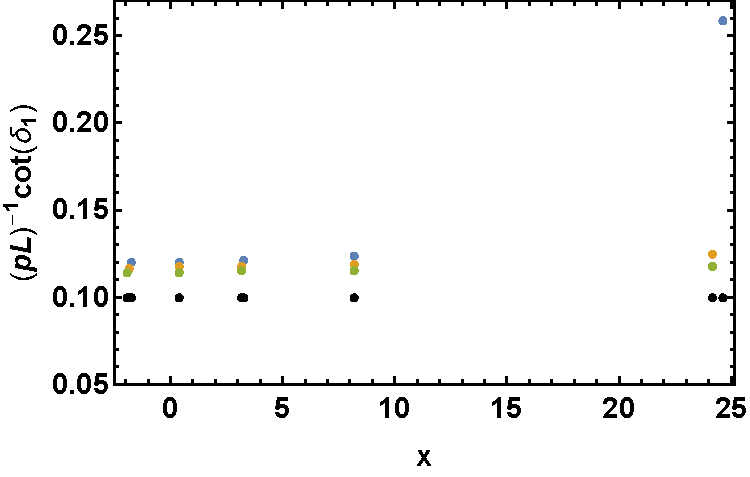
\includegraphics[width=.6\textwidth]{figure/luescher1d.pdf}
\caption{Results using non-continuum eigenvalues $x=p^2L^2/4\pi^2$ of the Schr\"odinger equation with $N=10$, 12, and 14.  The interaction was tuned such that $a_{10}/L=.1$.  The non-black points are obtained using $S^\bigcirc_1(x)$ with $N=10$ being furthest from a flat line and $N=14$ being closest.  The black points are obtained using $S^{\dispersion}_1(x)$  and exhibit the correct flat-line behavior.  Notice the offset between the colored and black points $x\le 0$.\label{fig:luescher1d}}
\end{figure}
